\documentclass{jlreq} 
%\usepackage{url} 
\usepackage{float}
\usepackage{graphicx} 
\usepackage{multicol}
\usepackage{ascmac}
\usepackage{siunitx}
\usepackage{listings}
\usepackage{xcolor}
\usepackage{amsmath}
%赤い枠が出ないようにhyperrefを読み込む 

\usepackage{fancyvrb}
\usepackage{hyperref}%pdfに赤い枠を出さない
\hypersetup{
  colorlinks=true,
  linkcolor=black,
  filecolor=magenta,
  urlcolor=blue,
  citecolor=black,
}

\lstnewenvironment{mylisting}[1][]%
  {\lstset{
    frame=single,
    basicstyle=\ttfamily\small,
    numbersep=6pt,
    tabsize=3,
    extendedchars=true,
    xleftmargin=17pt,
    framexleftmargin=17pt,
    breaklines=true,
    numbers=left,
    language=Matlab,  % ← ここで言語指定
    #1
  }}{}


\begin{document}

% --- 表紙 ---
\begin{titlepage}
  \centering
  \vspace{2cm}
  {\LARGE \bfseries システム提案書 \par}
  \vspace{1cm}
  {\LARGE \bfseries 香美市特化型配達サービス \par}
  \vspace{1cm}
   {\LARGE \bfseries Stellar Delivery \par}
  \vspace{3cm}
  %第2版
  {\Large 第2版 \par}
  %少し開けて作成日を入れる
  \vspace{4cm}
  {\Large \today \par}
  \vspace{0.5cm}
  {\LARGE \bfseries StellarWorks \par}
  \vfill
\end{titlepage}

\newpage

\tableofcontents
\newpage


\section{現状の課題}
\subsection{香美市の高齢者の割合}
高知県産業振興推進部統計分析課によると、令和5年の香美市の年齢別人口および割合は次のようになっている。

\begin{figure}[h]
  \centering
  \begin{minipage}{0.43\columnwidth}
    \centering
    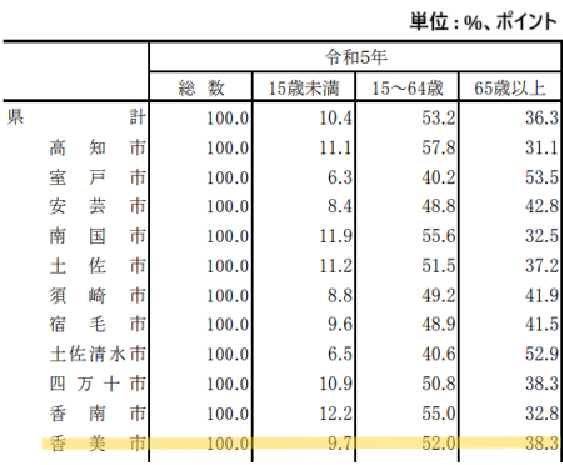
\includegraphics[width=\columnwidth]{population_rate.pdf}
    \caption{市町村別の年齢別人口}
    \label{fig:サンプルA}
  \end{minipage}
  \hspace{5mm}
  \begin{minipage}{0.43\columnwidth}
    \centering
    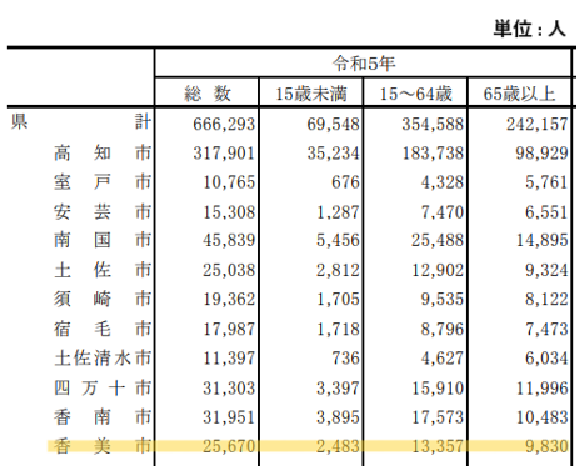
\includegraphics[width=\columnwidth]{population.pdf}
    \caption{市町村別の年齢別人口割合}
    \label{fig:サンプルB}
  \end{minipage}
\end{figure}

%年齢別人口(上位5位)のグラフをここに追加するかどうか?

この統計から、香美市の総人口は25,670人であり、そのうち高齢者(高齢者)は約9,800人で全体の4割近くを占めていることが分かる。また、香美市は高知県内の市町村の中でも65歳以上の人口が第5位に位置しており、県内でも特に高齢者人口が多いことが分かる。

今後も人口減少や少子高齢化の進行によって、高齢者の割合がさらに増加する可能性が高い。そのため、働き手となる世代が減少する一方で、生活支援を必要とする高齢者が増えるという問題と向き合っていかなければならない。

このような背景から、香美市では高齢者の生活を支える新たな仕組みづくりや、地域住民が安心して暮らせる環境整備が必要であると考えられる。特に、買い物や移動といった日常生活のサポート体制をどう確保するかが今後の重要な課題である。



\subsection{生活用品を確保する手段}
中山間地域を中心とした概ね50世帯未満の集落を対象に実施された「令和3年度高知県集落実態調査」によると、食料品などの生活必需品を確保する際に困難や課題を感じている人が全体の6割以上にのぼることが明らかになっている。
特に中山間地域では、「移動手段がない」「移動販売の頻度が少ない」といった問題が多く挙げられており、買い物環境の不便さが日常生活に大きな影響を及ぼしていることが分かる。
さらに、令和2年国勢調査を基にした集落調査データによれば、香美市では50世帯未満の小規模集落が全体の65.9\%を占めている。
このことから、香美市内においても同様に、移動手段の不足や移動販売の機会の少なさが深刻な課題となっていると考えられる。


\begin{figure}[h]
  \centering
  \begin{minipage}{0.43\columnwidth}
    \centering
    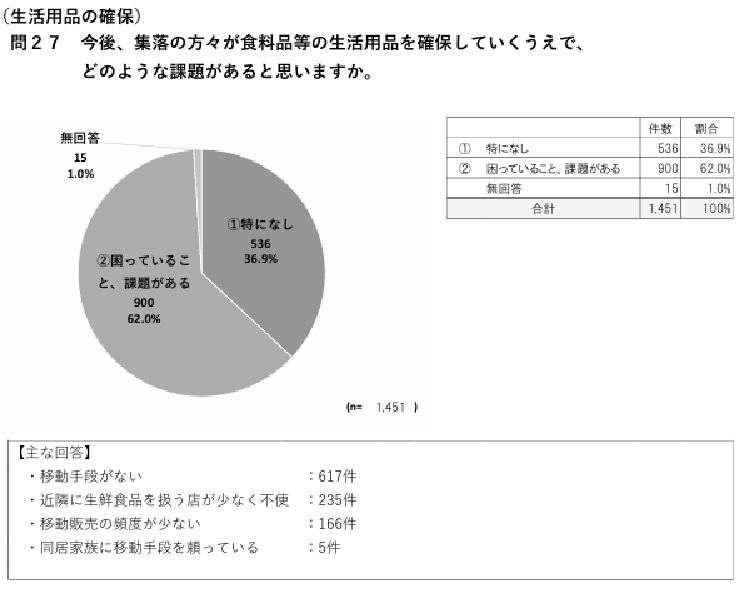
\includegraphics[width=\columnwidth]{get_food_graph.pdf}
    \caption{生活用品確保のための課題}
    \label{fig:get_food}
  \end{minipage}
  \hspace{5mm}
  \begin{minipage}{0.43\columnwidth}
    \centering
    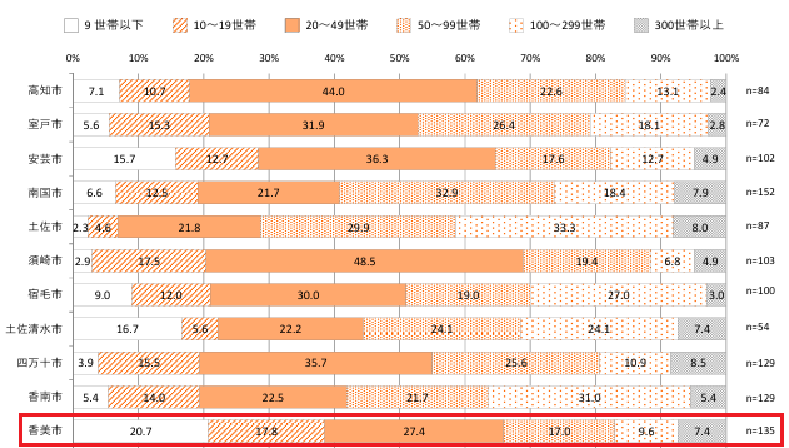
\includegraphics[width=\columnwidth]{市町村別世帯数別集落数の割合.pdf}
    \caption{香美市の世帯数別集落数の割合}
    \label{fig:市町村別世帯数別集落数の割合}
  \end{minipage}
\end{figure}

\subsection{移動手段の確保}

図 \ref{fig:免許}は、高知県における人口と運転免許証保有者数を示したものである。令和3年時点での免許保有者数は約45.5万人にのぼり、年齢別に見ると「45~49歳」が最も多く、次いで「70~74歳」の保有者が多いことが分かる。さらに、75歳以上の後期高齢者でも約4.7万人が免許を保有していることから、多くの高齢者が日常生活において自家用車を移動手段として利用している現状がうかがえる。
しかし、加齢に伴う身体機能の低下や認知機能の変化により、今後は運転の継続が困難となる高齢者が増加すると考えられる。その結果、自動車以外の移動手段を持たない高齢者が外出や買い物を行うことが難しくなり、生活用品の確保に苦労する人がさらに増える可能性が高い。


\begin{figure}[H]
  \centering
  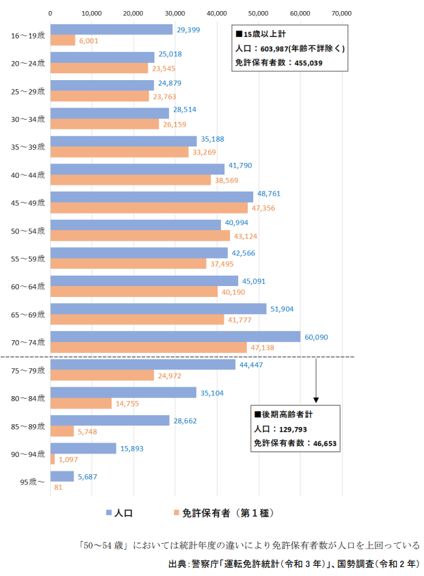
\includegraphics[width=0.5\textwidth]{免許証.png}
  \caption{高知県の人口と免許証保有者数}
  \label{fig:免許}
\end{figure}


\subsection{学生のバイト先の不足}
高知工科大学の学生102名にアンケート調査を行ったところ、図 \ref{fig:アンケート} のような結果が得られた。 
この結果から、全体の79.4\%の学生が香美市内で働くことを希望しているにも関わらず、実際に「香美市内にアルバイト先が十分にある」と感じている学生は12.8\%にとどまっていることが分かる。 
つまり、働く意欲を持つ学生に対して、香美市内ではそれを受け入れるだけの雇用機会が十分にはないという深刻な現状が明らかになっている。 
香美市は高知工科大学を有し、多くの学生が生活している地域であるにも関わらず、応募できる職種や店舗が限られており、「働きたいのに働けない」状況が常態化していると考えられる。 

\begin{figure}[h]
  \centering
  \begin{minipage}{0.43\columnwidth}
    \centering
    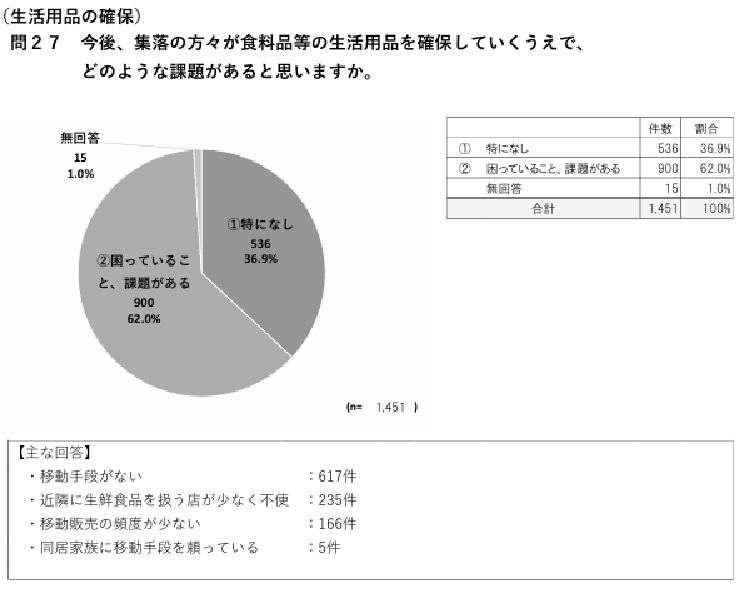
\includegraphics[width=\columnwidth]{get_food_graph.pdf}
  \end{minipage}
  \hspace{5mm}
  \begin{minipage}{0.43\columnwidth}
    \centering
    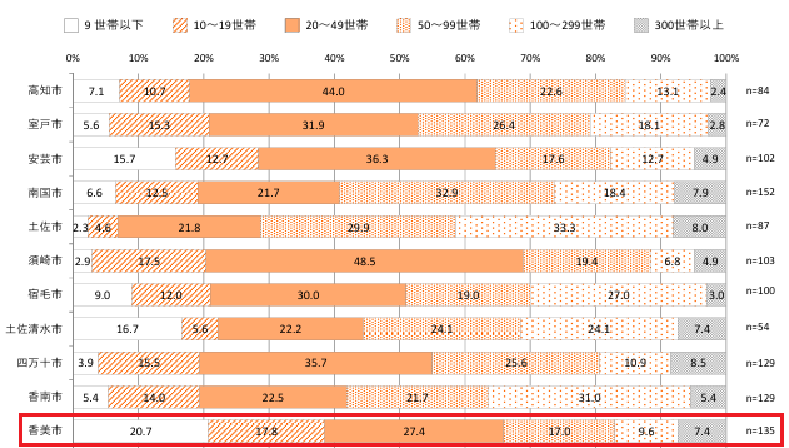
\includegraphics[width=\columnwidth]{市町村別世帯数別集落数の割合.pdf}
  \end{minipage}
  \caption{バイト先に関するアンケート調査結果}
  \label{fig:アンケート}
\end{figure}
%未完成


\section{課題解決のための提案}
上記の課題を踏まえ、高齢者が生活用品を手軽に確保でき、かつ学生の働き口を増やせる画期的な手段として、我々StellarWorksはインターネットに接続可能な端末から気軽に利用できる Stellar Delivery を提案する。
本アプリは、欲しいものを依頼すると、その商品をお店側と連携して学生が配達してくれるというものである。

\subsection{解決されると考えられる事象- 移動手段の確保問題}

小節1.2および1.3で述べたように、現在、多くの人々が生活用品を確保する際に「移動手段がない」「移動販売が少ない」といった課題に直面しており、このような状況は、少子高齢化の進行や地域交通網の縮小に伴い、今後さらに深刻化することが予想される。

そこで、我々が考案したシステムを活用することで、利用者は自宅にいながら簡単な操作で必要なものを注文し、配達を受けることが可能となる。
これにより、移動の負担を大幅に軽減し、買い物困難者の生活の質向上に寄与できると考えられる。

さらに本システムは、高齢者だけでなく、体調不良や病気、事故、子育てなどの理由で外出が難しい人々にとっても有効な支援手段となりうると考えられる。 

また、高知工科大学の学生102名にアンケート調査を行い、「我々が提案するデリバリーサービスを依頼側として使用したいか」という質問をしたところ、全体の77.4\%から肯定的な意見が得られた。(図 \ref{fig:アンケート2}) 
このため学生からの需要も十分にあると考えられる。 

\begin{figure}[H]
  \centering
  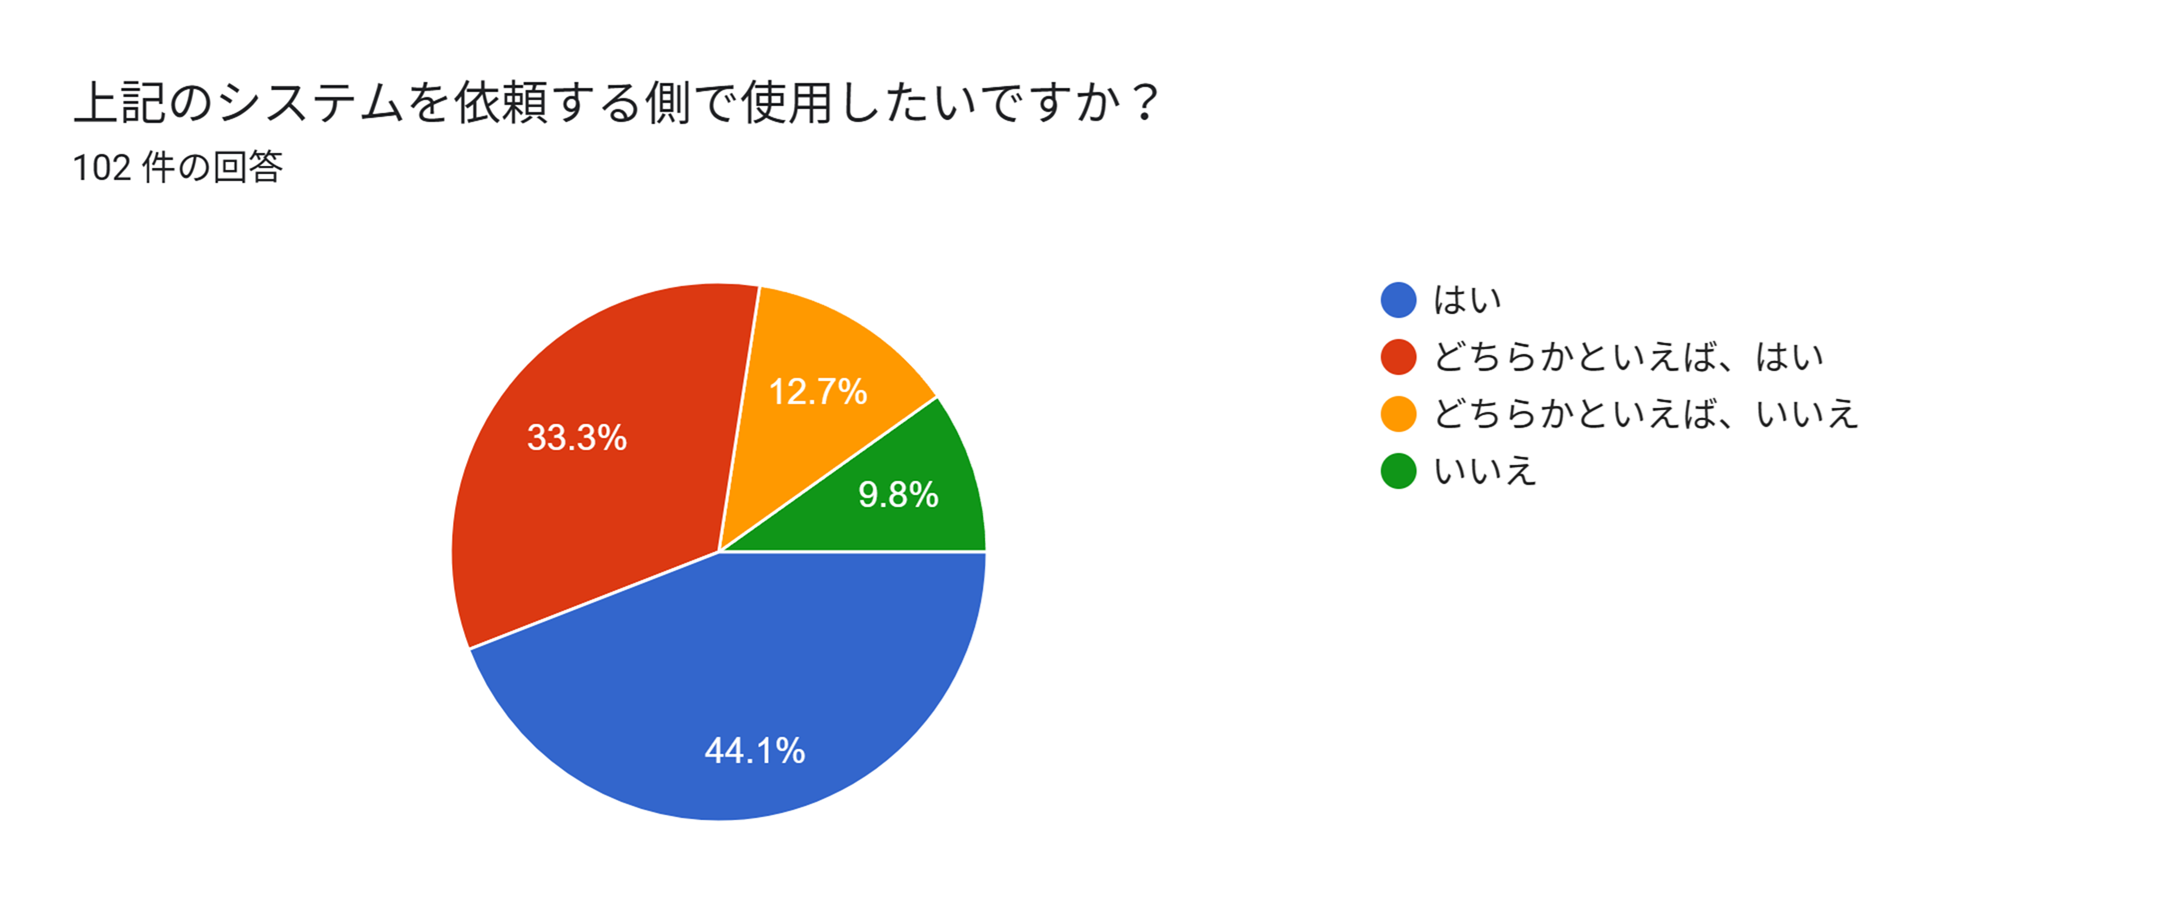
\includegraphics[width=0.75\textwidth]{依頼する側として使用したいか_アンケート結果.png}
  \caption{依頼する側として使用したいかのアンケート調査結果}
  \label{fig:アンケート2}
\end{figure}

%生活用品の確保問題がコメントアウトされている理由
%移動手段の確保問題と内容が被る可能性があるため、それぞれで分けるよりも1つにまとめる方が良いかも

%\subsection{解決されると考えられる事象- 生活用品の確保問題}



\subsection{解決されると考えられる事象- 香美市のアルバイト先の枯渇問題}
%アンケート結果より記述された小節1.3を参考
小節1.4で述べたように、現在の香美市では、学生が働けるアルバイト先が少なく、仕事を見つけづらい状況が続いている。
これは地域の店舗数の減少や人員の削減などが原因で、学生にとっても地域にとっても大きな課題となっている。
そこで、我々が提案するシステムを活用することで、この問題を解消できる可能性があると考えられる。
このサービスでは、商品の配達を学生が担当できるため、新しいアルバイトの場を作り出すことができる。
また、学生にとっては空いた時間を使って働ける柔軟な働き方が可能となり、地域にとっても若者の活躍の場が増えることで活性化につながる。
こうした仕組みにより、香美市のアルバイト不足の問題を解決し、地域全体を元気にすることが期待される。





\section{機能概要・前提条件・制約事項}
\subsection{機能概要}

\subsubsection{配達側}

\begin{itemize}
  \item 会員機能
    \begin{itemize}
        \item 新規会員機能
        
        名前、性別、歳、住所、メールアドレス、電話番号、パスワードを登録し会員になる機能。また、新規会員登録の際に規約を提示し、規約に従う場合に新規登録を行う。ただし、パスワードは作成条件を つける。
        \item ログイン・ログアウト
        
        ログイン機能では、すでに会員である配達側がメールアドレス、パスワードを入力することによっ てアプリにログインをする。ログアウト機能では、アプリにログインしている会員が任意のタイミング でログアウトできる。パスワードを忘れた際などに、メールアドレスを入力することによってパスワー ドを再設定することが可能。
        \item 退会
        
        会員が任意のタイミングでアプリ会員から退会する機能。会員情報を完全に削除する。
        \item 会員情報確認
        
        会員ごとに存在するマイページを確認する機能。会員情報として登録している情報が表示される。
        \item 会員情報変更
        
        登録している会員情報を変更する機能。
        \item 履歴書情報記述機能
        
        求人に応募する場合に用いる履歴書を記述する機能。この機能は新規会員登録の場合にはスキップができ、後々記述することが可能。
        \item 問い合わせ機能
        
        この画面ではアプリの運営への問い合わせができ、操作方法等の質問をメール形式で送信することが可 能となっている。質問への回答はアプリ利用者が登録したメールアドレスへ送信される。
        \item パスワード変更機能
      
        パスワードを作成条件下で任意に変更する機能。
        
    \end{itemize}
  \item メディア機能
  \begin{itemize}
      \item 求人情報表示
      
      香美市内にある求人情報を表示する。一覧画面では、店舗名、店舗の住所、配達先の住所、配達物の情報、報酬額を表示する。一覧に表示する順序は、新着順で行う。

     %配達手段として、自転車以上が推奨のような表示があるといいかも
      
      \item タグ分け機能
      
      タグは地域(土佐山田、香北など)、商品のジャンル、配達希望時間、金額とする。タグ分け機能では、それぞれのタグを指定した際にそのタグ内容ごとに求人の表示を行う機能である。
      
      \item 求人検索機能
      
      求人情報一覧より、利用者が任意のワードを入力することでそのワードに該当する求人が表示される。
    
      
      \item 配達履歴機能
      
      配達側ユーザーが配達を完了した依頼の履歴を取得しておき、マイページにて閲覧する機 能。閲覧履歴ページにて情報を選択すると詳細ページへと進む。詳細ページでは店舗名、配達物の情報、報酬額、受注時刻、完了時刻を表示する。配達側ユーザーが配達を完了した依頼の履歴を取得しておき、マイページにて閲覧する機 能。閲覧履歴ページにて情報を選択すると詳細ページへと進む。詳細ページでは店舗名、配達物の情報、報酬額、受注時刻、完了時刻を表示する。
      \item 求人応募機能
      
      求人に対して応募を行う機能。このボタンを押すには履歴書情報をマイページより記入する必要があ り、記入していない状態で押すと履歴書情報記入ページへと進むこととする。ボタンを押すと店舗に対して配達ユーザーの履歴書情報、連絡先が送られ、店舗と配達ユーザー間の連絡 を行う。
  \end{itemize}
\end{itemize}


\subsubsection{依頼側}

\begin{itemize}
  \item 会員機能
    \begin{itemize}
        \item 新規会員機能
        
        名前、性別、歳、住所、メールアドレス、電話番号、パスワードを登録し会員になる機能。また、新規会員登録の際に規約を提示し、規約に従う場合に新規登録を行う。ただし、パスワードは作成条件を つける。
        \item ログイン・ログアウト
        
        ログイン機能では、すでに会員である配達側がメールアドレス、パスワードを入力することによっ てアプリにログインをする。ログアウト機能では、アプリにログインしている会員が任意のタイミング でログアウトできる。パスワードを忘れた際などに、メールアドレスを入力することによってパスワー ドを再設定することが可能。
        \item 退会
        
        会員が任意のタイミングでアプリ会員から退会する機能。会員情報を完全に削除する。
        \item 会員情報確認

        会員ごとに存在するマイページを確認する機能。会員情報として登録している情報が表示される。
        \item 会員情報変更
        
        登録している会員情報を変更する機能。
        \item 問い合わせ機能
        
        この画面ではアプリの運営への問い合わせができ、操作方法等の質問をメール形式で送信することが可 能となっている。質問への回答はアプリ利用者が登録したメールアドレスへ送信される。
        \item パスワード変更機能
        
        パスワードを作成条件下で任意に変更する機能。
        \item 店舗検索機能
        
        依頼者が任意のワードを入力し、そのワードに該当する店舗が表示・検索される。
        
        \item 商品検索機能
        
        依頼者が任意のワードを入力し、そのワードに該当する商品が表示・検索される。

        \item カート機能

        商品を選択すると一時的にカートに追加される。また、カート内にある商品の情報を閲覧することが可能である。そして、選択済みおよびカートに追加した商品を削除することが可能である。

        注文が完了された商品はカートから削除される。

        
        \item 注文確定機能
        
        カート内に追加された商品の注文を確定する。
        
        \item 配達先候補の住所登録・削除
        
        配達先として複数の住所を登録し、指定することが可能である。候補は3つまで登録・削除可能である。
        
        \item 配達状況
        配達状況は、依頼済み、配達受付完了、配達中、配達完了の4段階に分けられ、依頼者が現在の配達状況を確認できる。
    \end{itemize}
  
\end{itemize}



\subsubsection{店舗側}

\begin{itemize}
  \item 会員機能
    \begin{itemize}
        \item 店舗新規登録申し込み
        %住所入力の際に対応エリア内であるのかを判断してくれるといいな
        
        店舗新規登録申し込みでは店舗名、店舗所在地、飲食店営業許可書のファイルおよび写真、メールアドレスまたは電話番号を入力して申込を行う。

        \item 新規会員機能
        
        名前、性別、歳、住所、メールアドレス、電話番号、パスワードを登録し会員になる機能。また、新規会員登録の際に規約を提示し、規約に従う場合に新規登録を行う。ただし、パスワードは作成条件を つける。
        \item ログイン・ログアウト
        
        ログイン機能では、すでに会員である配達側がメールアドレス、パスワードを入力することによっ てアプリにログインをする。ログアウト機能では、アプリにログインしている会員が任意のタイミング でログアウトできる。パスワードを忘れた際などに、メールアドレスを入力することによってパスワー ドを再設定することが可能。
        \item 退会
        
        会員が任意のタイミングでアプリ会員から退会する機能。会員情報を完全に削除する。
        \item 会員情報確認
        
        会員ごとに存在するマイページを確認する機能。会員情報として登録している情報が表示される。
        \item 会員情報変更
        
        登録している会員情報を変更する機能。
        \item 問い合わせ機能
        
        この画面ではアプリの運営への問い合わせができ、操作方法等の質問をメール形式で送信することが可 能となっている。質問への回答はアプリ利用者が登録したメールアドレスへ送信される。
        \item パスワード変更機能
        
        パスワードを作成条件下で任意に変更する機能。
        \item メニュー情報登録機能
        
        商品名、対象の写真、価格、説明文、カテゴリ(野菜や肉など)を登録する機能。
        \item メニュー情報更新機能
        
        メニューの商品名、対象の写真、価格、説明文、カテゴリを更新する機能。
        \item メニュー情報削除機能
        
        登録されているメニューを任意のタイミングで削除する機能。

        \item 在庫更新機能
        
        メニューの在庫(販売中 or 売り切れ)を更新する機能。
    \end{itemize}
  
\end{itemize}

\subsection{管理者側}
%コピペで持ってきたから内容をいい感じに変える。

\begin{itemize}
  \item アカウント管理
    \begin{itemize}
        \item 依頼者アカウントの管理機能
        
        管理者は、依頼者のアカウントを登録・編集・削除することができる。また、商品の配達状況や注文履歴などの管理を行う。


        \item 配達員アカウント管理機能
        
        管理者は、配達員のアカウントを登録・編集・削除することが可能である。また、配達履歴の管理を行う。

        \item 店舗アカウント管理機能

        管理者は、店舗のアカウントを登録・編集・削除することが可能である。
        
        \item 管理者アカウントの管理

        他の管理者のアカウントを登録・編集・削除することが可能である。
        
        \item 注文管理機能
        
        管理者は、ユーザーからの問い合わせを受け取り表示することができる。

        \item 支払い額管理機能

        依頼者および店舗が支払う料金を管理する。また、配達員への報酬額を管理する。


    \end{itemize}
  
\end{itemize}

\subsection{前提条件}
 本システム提案書では以下の条件を前提条件とする。

 \begin{itemize}
  \item 利用者がインターネットに接続可能な端末(iOSまたはandroidに対応)を保有していること。
  \item 利用者が本アプリケーションの規約に同意済みであること。
  \item 本アプリケーションの使用には会員登録が必須であること。
\end{itemize}

店舗側は店舗申請を行う際、以下の出店条件を満たすこととする。

\begin{itemize}
  \item 対応エリア(香美市)内に店舗があること。
  \item 飲食店営業許可証があること。
\end{itemize}

\subsection{制約事項}
本システム提案書では以下の事項を制約事項とする。
\begin{itemize}
    \item 利用者の住所や氏名などの個人情報の漏洩を防ぐ仕様であること。
    \item 管理者側による投稿の削除・規制が行える仕様であること。
\end{itemize}


\section{情報・金銭の流れ}
\subsection{情報の流れ}
本システムは、管理者サーバー・データベースを中心に、利用者(依頼者)・配達員・サービス加盟店(店舗)によって構成されている。図\ref{system}~図\ref{money}に情報および金銭の流れを示す。図6,7は情報の流れ、図8は金銭の流れを表している。
本システムでは、利用者がアプリ上で商品を注文すると、注文情報がサーバーを介して店舗および配達員に送信される。配達員は受注内容に基づき店舗から商品を受け取り、指定の配達先まで配送を行う。配達完了後、店舗および配達員はそれぞれシステムに配送完了報告を送信し、管理サーバーで取引が確定する。

\begin{figure}[H]
  \centering
  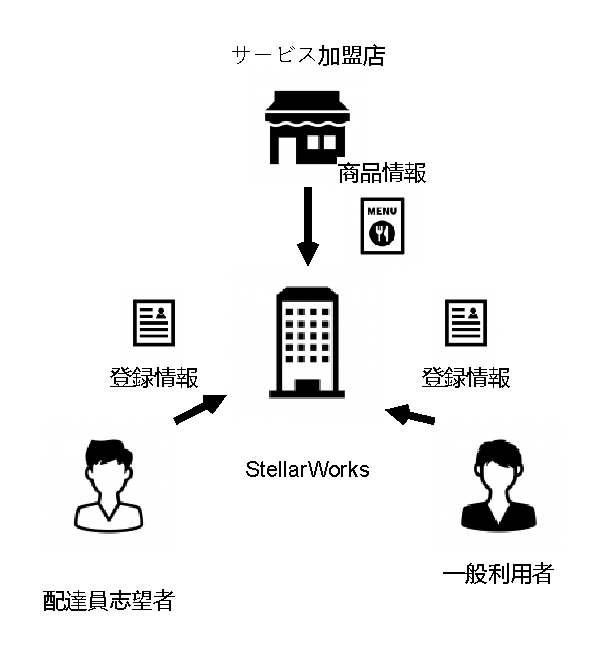
\includegraphics[width=0.5\textwidth]{情報の流れ.drawio.pdf}
  \caption{情報の流れ: 情報登録}
  \label{system}
\end{figure}

\begin{figure}[H]
  \centering
  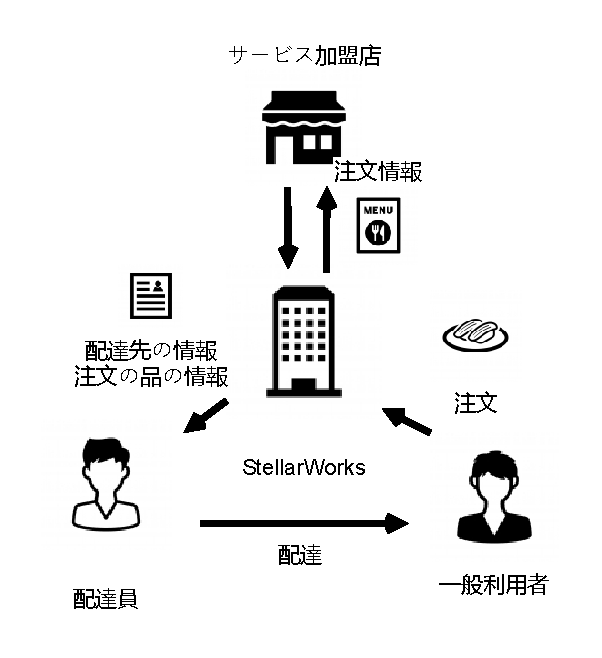
\includegraphics[width=0.5\textwidth]{流れ.drawio.pdf}
  \caption{情報の流れ: 注文から配達まで}
  \label{oder}
\end{figure}


\subsection{金銭の流れ}
本システムの金銭の流れは以下の通りである。
支払い方式は銀行振り込みによる月末一括精算方式を採用している。利用者(依頼者)は、当月内の利用分について月末にまとめて銀行振り込みで支払いを行う。
また、クレジットカードを用いたオンライン決済システムも導入しており、利用者はアプリ上でクレジットカード情報またはkamicaなどの情報を登録し、月末に自動的に決済が行われる仕組みとなっている。
運営側は決済代行システムを通じて支払いを一元管理し、店舗・配達員への報酬支払いを翌月初めに一括処理する。
これにより、個々の取引ごとに発生していた送金処理を効率化し、運用コストを削減している。
また、配達員は商品を受け取る際に自らの手持ち資金を使用しないため、商品が売り切れなどの不測の事態が発生しても払い戻しが三者間で発生しない仕組みとなっている。
利用者は返金や精算の手間をかけることなく、快適にシステムを利用できる。
このように、本システムは銀行振り込み機能を用いることで、取引の透明性と効率性を両立した金銭管理体制を実現している。
\begin{figure}[H]
  \centering
  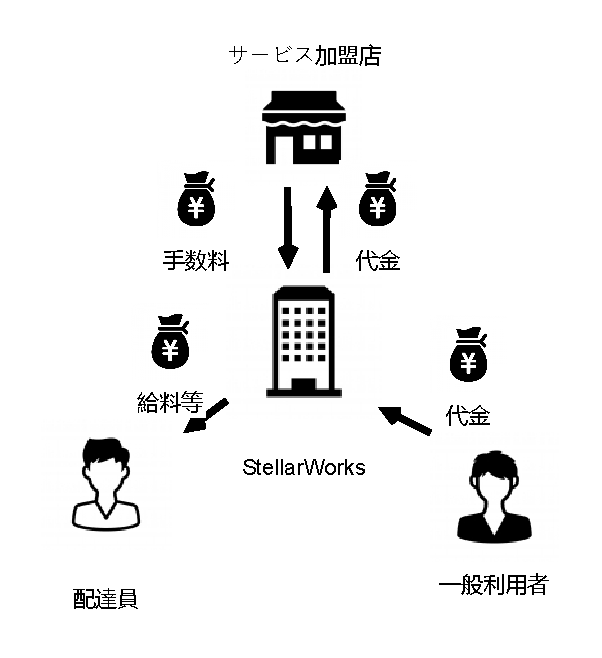
\includegraphics[width=0.5\textwidth]{お金の流れ1.pdf}
  \caption{金銭の流れ}
  \label{money}
\end{figure}


\section{想定する利用者}
本システムの利用者を以下に示す。
\begin{itemize}
\item 配達員として働きたい利用者

\item 食事を注文したい利用者

\item 注文を受けたい店舗側の利用者
\end{itemize}

\section{ハードウェア構成・ソフトウェア構成}
\subsection{ハードウェア構成}
%表を用いて書きたい
本システムのハードウェア構成を表\ref{tab:hardware_configuration}に示す。
\begin{table}[H]
 \centering
 \begin{tabular}{|c|c|c|c|}
 \hline
 項目 & 種類 & 数量 & 備考\\
 \hline
 メインサーバー & レンタルサーバー & 1 & \\
 \hline
 データベースサーバー & レンタルサーバー & 1 & \\
 \hline
 管理者端末 & デスクトップPC & 1 & \\
 \hline
 ユーザー端末 & スマートフォン & 利用者数 & \\
    \hline
 \end{tabular}
 \caption{ハードウェア構成}
 \label{tab:hardware_configuration}
\end{table}

\subsection{ソフトウェア構成}
本システムのソフトウェア構成を表\ref{tab:software_configuration}に示す。
\begin{table}[H]
 \centering
 \begin{tabular}{|c|c|}
 \hline
 ソフトウェア & 備考\\
 \hline
 バックエンド & FastAPI\\
 \hline
 フロントエンド & Flutter\\
 \hline
 Webサーバ & Nginx\\
 \hline
 データベース管理システム & MySQL\\
 \hline
 管理者端末 & Ubuntu 22.04\\
 \hline
 利用者端末 & Android, iOS\\
 \hline
 \end{tabular}
 \caption{ソフトウェア構成}
 \label{tab:software_configuration}
\end{table}

\section{運用・保守}
システムの運用・保守に関しては以下の通りである。
\subsection{運用}
\begin{itemize}
    \item 利用者アカウントの管理
    \item 求人情報や応募情報の登録・承認・公開管理
    \item システム稼働状況の定期的な監視
    \item 問い合わせ対応
    \item 利用者向けの操作マニュアル・FAQの整備
    %金澤 10/15(水) 配達可能時間や注文受付時間はどうするのか?
\end{itemize}
\subsection{保守}
\begin{itemize}
    \item 不具合発生時の原因調査及び修正対応
    \item OS等のバージョンアップ対応
    \item セキュリティ対策
    \item 機能改善や新規要望に基づく改修の検討・実装
\end{itemize}

\section{費用対効果}
\subsection{効果}
本システムの導入により、地域住民は多様な商品を手軽かつ迅速に購入できるようになる。
香美市の個人経営店舗を支援し、地域経済の活性化を促進することを目的としている。
ユーザーはスマートフォンを活用し、時間や場所を問わず商品を購入できるため、利便性が大幅に向上する。
店舗側もオンライン販売の拡大により、売上増加が期待できる。
また、システムは高齢者にも使いやすいユーザーフレンドリーなインターフェースを備えており、幅広い世代が安心して利用できる。
さらに、大学生のアルバイト機会も創出し、地域の若者の雇用促進と社会活性化にも貢献する。



\subsection{収益}
本システムの収益は、Uber Eatsの収益構造を参考にしており、
「店舗手数料」「配達料金の一部」「ユーザーサービス料」の3つを主な柱としている。
登録店舗は、アプリ上で注文が発生するたびに、注文金額の30%を手数料として運営側に支払う。
平均お弁当価格を700円とした場合、1件あたりの手数料収益は210円となる。
ユーザーは配達距離に応じて「基本料金150円+距離50円/km」を支払う。
平均配達距離を2kmとすると配達料金は250円となり、そのうち30%(75円)を運営側収益として受け取る。
残りの70%は配達員報酬とする。
各注文につき、70円の固定手数料をユーザーから徴収し、これを全額収益とする。

年間件(1日あたり約220件)の注文を想定すると、
\[
年間総収益=355円 \times 約80,000件 = 28,400,000円 となる。
\]
これを5年間運用すると
 \[
 28,400,000\text{ 円} \times 5\text{ 年} = 142,000,000\text{ 円}
 \]

\subsection{費用}
本システムの主な費用は、サーバー運用・開発保守・プロモーション・配達員報酬などである。
以下に年間費用をまとめる。
\begin{table}[H]
\centering
\caption{初期費用}
\begin{tabular}{|c|c|c|c|}
\hline
項目 & 単価 (円) & 数量 & 金額 (円) \\
\hline
管理者用端末 & 100,000 & 6 & 600,000 \\
\hline
\end{tabular}
\end{table}

また、運用費用は以下の通りとなる。

\begin{table}[H]
\centering
\caption{運用費用}
\begin{tabular}{|c|c|c|c|}
\hline
項目 & 単価 (円) & 数量 & 金額 (円) \\
\hline
人件費 & 4,000,000 / 年 & 6 & 24,000,000 \\
\hline
サーバーレンタル & 36,000 / 年 & 1 & 36,000 \\
\hline
\end{tabular}
\end{table}

よって、5年間の費用合計は以下のようになる。

\[
(24,000,000\text{ 円} + 36,000\text{ 円}) \times 5 = 120,180,000\text{ 円}
\]
\[
120,180,000\text{ 円} + 600,000\text{ 円} = \boxed{120,780,000\text{ 円}}
\]

\subsection{利益}
このアプリを5年間運用した利益は以下のようになる
\[
142,000,000\text{ 円}-120,780,000\text{ 円} = 21,220,000\text{ 円}
\]

\section{開発体制と工程計画}
本システムの開発には高知工科大学情報学群のStellerworksのプログラマー6人で行う。
本システムの開発工程は以下に示す通りである。
\begin{figure}[H]
  \centering
  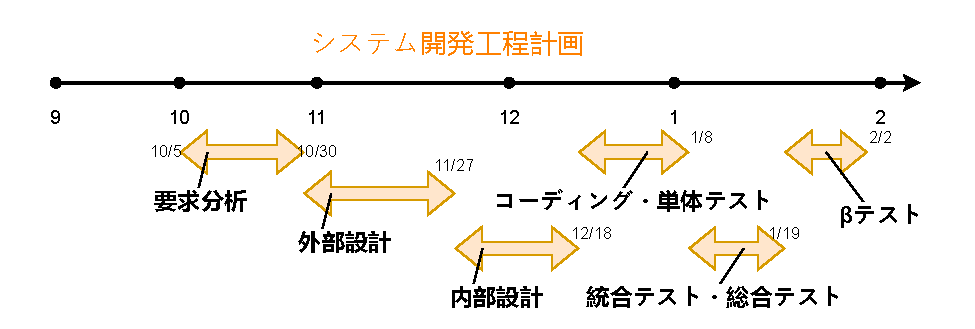
\includegraphics[width=0.9\textwidth]{開発計画.pdf}
  \caption{開発工程計画}
  \label{gantt}
\end{figure}

\section{システムアピールポイント}
\begin{itemize}
  \item データ活用によるマーケティング支援
  \item 地域密着型プラットフォーム
  \item 利用者・店舗双方にメリット
  \item 低コストで導入可能
\end{itemize}   

\begin{thebibliography}{9}

\bibitem{kochi_population}
高知県産業振興推進部統計分析課,
「高知県の推移人口年報(令和5年)」,
\url{https://www.pref.kochi.lg.jp/doc/t-suikei/file_contents/r05_nennpou.pdf}

\bibitem{kochi_transport}
高知県地域公共交通活性化協議会,
「高知県地域公共交通計画」,
\url{https://www.pref.kochi.lg.jp/doc/2023033000302/file_contents/file_20233304202123_1.pdf}

\bibitem{kochi_village}
高知県庁,
「令和3年度 高知県集落調査」,
\url{https://www.pref.kochi.lg.jp/doc/2022032900286/file_contents/04_r3_shuurakude-tatyousa.pdf}

\bibitem{ubereats_model}
しごとナビ,
「Uber Eatsのビジネスモデルとは?」,
\url{https://shigoto.work/ubereats-business-model}

\end{thebibliography}


\end{document}

